\usepackage{stmaryrd}

\newcommand{\E}{\mathbf{E}}
\newcommand{\B}{\mathbf{B}}
\renewcommand{\H}{\mathbf{H}}
\newcommand{\D}{\mathbf{D}}

\newcommand{\J}{\mathbf{J}}
\newcommand{\Jphat}{\hat{\J}_p}
\newcommand{\Jpol}{\J^p}
\newcommand{\JpolScalar}{J^p}
\newcommand{\plasfreq}{\omega_p}
\newcommand{\plasfreqtilde}{\tilde{\omega}_p}

\newcommand{\xbf}{\mathbf{x}}

\newcommand{\xbftilde}{\tilde{\mathbf{x}}}
\newcommand{\xtilde}{\tilde{x}}
\newcommand{\nablatilde}{\tilde{\nabla}}
\newcommand{\Etilde}{\tilde{\mathbf{E}}}
\newcommand{\Btilde}{\tilde{\mathbf{B}}}
\newcommand{\Htilde}{\tilde{\mathbf{H}}}
\newcommand{\Dtilde}{\tilde{\mathbf{D}}}
\newcommand{\Jtilde}{\tilde{\mathbf{J}}}
\newcommand{\Jtildep}{\tilde{\mathbf{J}}_P}
\newcommand{\ttilde}{\tilde{t}}
\renewcommand{\t}{t}
\newcommand{\omegatilde}{\tilde{\omega}}
\newcommand{\gammatilde}{\tilde{\gamma}}

\newcommand{\bigO}{\mathcal{O}}
\newcommand{\Epsilon}{\mathcal{E}}

\newcommand{\weightfunc}{\mathbf{W}}
\newcommand{\R}{\mathbf{R}}
\newcommand{\ut}{\frac{\partial \mathbf{U}}{\partial t}}
\newcommand{\fk}{\frac{\partial \mathbf{F_k (\mathbf{U})} }{\partial x_k}}

% Temporal discretisation
\newcommand{\CFLCondition}{C}
\newcommand{\speedoflightCFL}{c}
\newcommand{\minElemSize}{h}

% --------------------------------------------------------------------------------------------- %
% Words
% --------------------------------------------------------------------------------------------- %

\newcommand{\SilverMuller}{Silver-M\"uller}

% --------------------------------------------------------------------------------------------- %
% General
% --------------------------------------------------------------------------------------------- %

\newcommand{\Real}{\mathbb{R}}
\newcommand{\RealPart}{\textrm{Re}}
\newcommand{\ImagPart}{\textrm{Im}}
\newcommand{\norm}[1]{\left\lVert#1\right\rVert}
\newcommand{\zerov}{\mathbf{0}_3}
\newcommand{\zerom}{\mathbf{0}_{3\times3}}
\newcommand{\IdentityVect}{\mathbf{I}_3}
\newcommand{\IdentityMatrix}{\mathbf{I}}
\newcommand{\0}{\bm{0}}


% Indicies
\newcommand{\nen}  {\ensuremath{\texttt{n}_{\texttt{en}}}}
\newcommand{\nef}  {\ensuremath{\texttt{n}_{\texttt{ef}}}}
\newcommand{\nfn}  {\ensuremath{\texttt{n}_{\texttt{fn}}}}
\newcommand{\nsd}  {\ensuremath{\texttt{n}_{\texttt{sd}}}}
\newcommand{\nip}  {\ensuremath{\texttt{n}_{\texttt{eq}}}}
\newcommand{\nipF}  {\ensuremath{\texttt{n}_{\texttt{fq}}}}
\newcommand{\ndof} {\ensuremath{\texttt{n}_{\texttt{dof}}}}
\newcommand{\nel}  {\ensuremath{\texttt{n}_{\texttt{el}}}}
\newcommand{\nT}  {\ensuremath{\texttt{n}_{\texttt{T}}}}
\newcommand{\nnode}  {\ensuremath{\texttt{n}_{\texttt{node}}}}

% --------------------------------------------------------------------------------------------- %
% General Physics
% --------------------------------------------------------------------------------------------- %

\newcommand{\speedoflight}{c}

% --------------------------------------------------------------------------------------------- %
% Physical Problem
% --------------------------------------------------------------------------------------------- %

% conservation form maxwells
\newcommand{\USoltn}{\mathbf{U}}
\newcommand{\Flux}{\mathbf{F}}
\newcommand{\maxwellSource}{\mathbf{S}}
\newcommand{\eps}{\varepsilon}

% Quasilinear form
\newcommand{\A}{\mathbf{A}}
\newcommand{\Ak}{\A_\mathbf{k}}
\newcommand{\Asource}{\A_s}
\newcommand{\Acomb}{\A^{s}}
\newcommand{\RQuasiL}{\mathbf{R}}
\newcommand{\RTot}{\mathbf{R}^{s}}

% Quasilinear form TE/TM
\newcommand{\Jnormalised}[1]{J_{#1}^*} % scalar

% Compact Form
\newcommand{\waveNumberVectZ}{\mathbf{k}_z}
\newcommand{\waveNumberZ}{k_z}
\newcommand{\phase}{\phi}

% integral formulation of Maxwell's equations
\newcommand{\vectdl}{\mathrm{d}\boldsymbol{\ell}}
\newcommand{\vectdS}{\mathrm{d}\mathbf{S}}
\newcommand{\Vol}{V}
\newcommand{\dV}{\mathrm{d}V}

% Physical Problem - dimensionless units
\newcommand{\czero}{c_0}
\newcommand{\charLen}{l}
\newcommand{\intImpFS}{\sqrt{\frac{\mu_0}{\eps_0}}} % ininsic impedence free space (\eta_0)

% Constitutive equations
\newcommand{\ElecSuccept}{\chi}
\newcommand{\MagSuccept}{\chi^{m}}
\newcommand{\Ptilde}{\tilde{\mathbf{P}}}
\newcommand{\Mtilde}{\tilde{\mathbf{M}}}

% Drude model - ADE
\newcommand{\PtildeInf}{\tilde{\mathbf{P}}_{\infty}}
\newcommand{\PtildeElec}{\tilde{\mathbf{P}}_P}
\newcommand{\PtildeInfFreq}{\hat{\tilde{\mathbf{P}}}_{\infty}}
\newcommand{\PtildeElecFreq}{\hat{\tilde{\mathbf{P}}}_P}
\newcommand{\ElecSucceptInf}{\chi_{\infty}}
\newcommand{\DInf}{\D_{\infty}}
\newcommand{\DtildeInf}{\tilde{\D}_{\infty}}

% Drude Model - mechanical
\newcommand{\xdispelecvect}{\tilde{\mathbf{x}}_e}
\newcommand{\EappliedDrude}{\tilde{\mathbf{E}}_{app}}

% Material interfaces
\newcommand{\matinterfacedomain}{\Omega}
% Helmholtz
\newcommand{\EHelm}{\E_0}
\newcommand{\HHelm}{\H_0}

% Modes
\newcommand{\TEz}{\textrm{TE}_{z}}
\newcommand{\TMz}{\textrm{TM}_{z}}

% --------------------------------------------------------------------------------------------- %
% DG Method
% --------------------------------------------------------------------------------------------- %

% weak form
\newcommand{\TFComp}{W} % test function
\newcommand{\TF}{\mathbf{\TFComp}}
\newcommand{\RTotNorm}{\RTot_{\mathbf{n}}}
\newcommand{\Ue}{\mathbf{U}_e}
\newcommand{\Uout}{\mathbf{U}_e^{\textrm{out}}}
\newcommand{\physicalDomain}{\Omega}
\newcommand{\physicalDomainBoundary}{\partial \physicalDomain}
\newcommand{\elemindex}{i}
\newcommand{\elemIndexed}{\physicalDomain_\elemindex}
\newcommand{\anotherelemindex}{j}
\newcommand{\anotherelem}{\physicalDomain_\anotherelemindex}
\newcommand{\approximationSpaceSpatial}{\bm{\mathcal{V}}}
\newcommand{\approximationSpaceTotal}{\mathcal{C}}
\newcommand{\genericElement}{\physicalDomain_e}
\newcommand{\periodOfApproximation}{T}
\newcommand{\barelemindexed}{\overline{\physicalDomain}_\elemindex}
\newcommand{\bardomain}{\overline{\physicalDomain}}
\newcommand{\delem}{d\Omega}
\newcommand{\uet}{\frac{\partial \Ue}{\partial t}}
\newcommand{\elemtracegenericelement}{\Gamma_e}
\newcommand{\delemtrace}{d\Gamma}
\newcommand{\NormalFlux}{\mathbf{\Flux_n}}
\newcommand{\outnormalcoeff}{n}
\newcommand{\outnormalcoeffcomp}{k}
\newcommand{\outnormalcoeffk}{\outnormalcoeff_{\outnormalcoeffcomp}}
\newcommand{\outnormalvector}{\hat{\mathbf{\outnormalcoeff}}}
\newcommand{\NumFlux}{\tilde{\Flux}}
\newcommand{\NormalFluxPositiveEigenvalues}{\NormalFlux^+}
\newcommand{\NormalFluxNegativeEigenvalues}{\NormalFlux^-}
\newcommand{\anyVector}{\mathbf{v}}
\newcommand{\xk}{x_k}

% Spaces
\newcommand{\LTwo}{\mathcal{L}^2(\Omega)}
\newcommand{\LTwoV}{\bm{\mathcal{L}}^2(\Omega)}
\newcommand{\Hcurl}{\bm{\mathcal{H}}(\textbf{curl},\Omega)}
\newcommand{\HcurlZero}{\bm{\mathcal{H}}_0(\textbf{curl},\Omega)}

% Quasilinear A
\newcommand{\an}{a_n}
\newcommand{\An}{\A_\mathbf{n}}
\newcommand{\AnPlus}{\An^{+}}
\newcommand{\AnMinus}{\An^{-}}
\newcommand{\AnMinusU}{\AnMinus \JumpU}
\newcommand{\AnMinusUSymbol}{\Flux^{\textrm{diff}}}
\newcommand{\modAnSubMatrix}{\mathbf{T}}
\newcommand{\nvect}{\mathbf{n}}

\newcommand{\bm}[1]{\boldsymbol{#1}}

\newcommand{\Jump}[1]{\llbracket #1 \rrbracket}
\newcommand{\JumpU}{\Jump{\USoltn}} % TODO - is this USoltn or UVect???
\newcommand{\JumpE}{\Jump{\E}}
\newcommand{\JumpH}{\Jump{\H}}

\newcommand{\LMat}[1]{#1^l}
\newcommand{\RMat}[1]{#1^r}
\newcommand{\LStarSymbol}{*}
\newcommand{\RStarSymbol}{**}
\newcommand{\LStarMat}[1]{#1^\LStarSymbol}
\newcommand{\RStarMat}[1]{#1^{\RStarSymbol}}
\newcommand{\SurfMat}[1]{#1^s}

\newcommand{\epsL}{\LMat{\eps}}
\newcommand{\epsR}{\RMat{\eps}}
\newcommand{\muL}{\LMat{\mu}}
\newcommand{\muR}{\RMat{\mu}}
\newcommand{\speedoflightleft}{\LMat{\speedoflight}}
\newcommand{\speedoflightright}{\RMat{\speedoflight}}

% --------------------------------------------------------------------------------------------- %
% DG Method Boundary Conditions
% --------------------------------------------------------------------------------------------- %

\newcommand{\UFieldComp}{V}
\newcommand{\UField}{\mathbf{\UFieldComp}}
\newcommand{\alphaGeneral}{\alpha}
\newcommand{\micoeff}{m} % material interface coeff
\newcommand{\micoeffL}{\LMat{\micoeff}} % material interface coeff
\newcommand{\micoeffR}{\RMat{\micoeff}} % material interface coeff
\newcommand{\micoeffinv}{n} % material interface coeff
\newcommand{\micoeffinvL}{\LMat{n}}
\newcommand{\micoeffinvR}{\LMat{n}}

% --------------------------------------------------------------------------------------------- %
% DG Method Discretisation
% --------------------------------------------------------------------------------------------- %

% Choice of Numerical Flux
\newcommand{\AnMod}{\An^{\parallel}}
\newcommand{\AnDiagP}{\mathbf{P}}
\newcommand{\AnDiag}{\mathbf{\Lambda}}
\newcommand{\AnDiagStar}{\mathbf{\Lambda}^{*}}
\newcommand{\AnDiagPInv}{\mathbf{P}^{-1}}

% Elemental Matrices
\newcommand{\MassMatrix}{\bm{M}_{ij}}
\newcommand{\MassMatrixFace}{\mathbf{M}^{\textrm{face}}_{ij}}
\newcommand{\MassMatrixAffine}{\mathbf{m}}
\newcommand{\MassMatrixFaceAffine}{\mathbf{m}^{\textrm{face}}}

\newcommand{\ConvectionMatrix}{\mathbf{C}^{k}_{ij}}
\newcommand{\ConvectionMatrixAffine}{\mathbf{c}^k}

% Might want to change
\newcommand{\faceindex}{m}
\newcommand{\discretisedWeakForm}[1]{
  \sum_{j=1}^{\nen}
  \MassMatrix
  \IdentityMatrix
  \dodet{\UVect_j}
+
  \sum_{j=1}^{\nen}
  \left( \ConvectionMatrix \Ak \right) \UVect_j
-
  \sum_{\faceindex=1}^{#1}
  \MassMatrixFace
  \AnMinus
  \Jump{\UVect_j}
 -
  \sum_{j=1}^{\nen}
  \MassMatrix
  \Asource
  \UVect_j
= 0
\; \; \forall \; i \; \in \; 1...\nen,
}

% Shape and Test functions
\newcommand{\SF}{N}

\newcommand{\JumpUVectUnkowns}{\llbracket \UVect \rrbracket}
\newcommand{\JumpUCoeffVectUnknownsWithIndex}[1]{\llbracket \UVect_{#1} \rrbracket}
\newcommand{\UVect}{\bm{U}}
\newcommand{\FluxDiv}{\Flux^{\elem}}

% Spatial Discretisation
\newcommand{\USoltnApprox}{\mathbf{U}_h}

% Reference Element
\newcommand{\IsoMapping}{\bm{\phi}}
\newcommand{\refelem}{\widehat{\physicalDomain}}
\newcommand{\meshelem}{\genericElement^{h}}
\newcommand{\meshelemtrace}{\Gamma^{h}_e}
\newcommand{\refElemCoords}{\mathbf{\xi}}
\newcommand{\refelemtrace}{\partial \IsoMapping}
\newcommand{\drefelemtrace}{d\Gamma_{\IsoMapping}}
\newcommand{\drefelem}{d\Omega_{\IsoMapping}}
\newcommand{\Jacobian}{\mathbf{J}_{\IsoMapping}}
\newcommand{\JacobianFace}{\mathbf{J}^{\textrm{face}}_{\IsoMapping}}
\newcommand{\refFace}{\widehat{\Gamma}}
\newcommand{\face}{\Gamma_e}

% Summations
\newcommand{\sumNen}{\sum_{j=1}^{\nen}}
\newcommand{\sumNfn}{\sum_{j=1}^{\nfn}}
\newcommand{\sumNsdK}{\sum_{k=1}^{\nsd}}
\newcommand{\sumNsdL}{\sum_{l=1}^{\nsd}}

% referential coordinates
\newcommand{\xiV}{\bm{\xi}}
\newcommand{\xCoord}{\bm{x}}
\newcommand{\nodalCoordinatesOfElement}{\xCoord_j}
\newcommand{\Uh}{\USoltn_{h}}

% Time integration
\newcommand{\Residual}{\bm{R}}
\newcommand{\ResidualInv}{\hat{\bm{R}}}
\newcommand{\MassMatrixInv}{\MassMatrix^{-1}}
\newcommand{\ResidualInvContrib}[1]{\ResidualInv^{(#1)}}

% --------------------------------------------------------------------------------------------- %
% PDEs and ODEs
% --------------------------------------------------------------------------------------------- %

\newcommand{\dpart}[2]{\frac{\partial #1}{\partial #2}}
\newcommand{\dpartt}[1]{\frac{\partial #1}{\partial t}}
\newcommand{\ddpartt}[1]{\frac{\partial^2 #1}{\partial t^2}}
\newcommand{\dpartttilde}[1]{\frac{\partial #1}{\partial \tilde{t} }}
\newcommand{\dpartx}[1]{\frac{\partial #1}{\partial x}}
\newcommand{\dpartxtilde}[1]{\frac{\partial #1}{\partial \tilde{x}}}

\newcommand{\dode}[2]{\frac{d #1}{d#2}}
\newcommand{\dodet}[1]{\frac{d #1}{d t}}
\newcommand{\dodett}[1]{\frac{d^2 #1}{d t^2}}
\newcommand{\dodettilde}[1]{\frac{d #1}{d \tilde{t}}}
\newcommand{\dodex}[1]{\frac{d #1}{d x}}
\newcommand{\dodextilde}[1]{\frac{d #1}{d \tilde{x}}}
% --------------------------------------------------------------------------------------------- %
% Figures
% --------------------------------------------------------------------------------------------- %

\newcommand{\singleFigure}[3]{
\begin{figure}[htbp!]
  \begin{center}
    \includegraphics[width=\textwidth]{Figures/#1}
  \end{center}
  \caption{#2}
  \label{fig:#3}
\end{figure}
}

\newcommand{\FigTwoByOne}[6]{
\centering
\begin{subfigure}{0.495\textwidth}
  \centering
  \includegraphics[width=\textwidth]{Figures/#1}
  \caption{#3}
  \label{fig:#5}
\end{subfigure} %
\begin{subfigure}{0.495\textwidth}
  \centering
  \includegraphics[width=\textwidth]{Figures/#2}
  \caption{#4}
  \label{fig:#6}
\end{subfigure}
}

\newcommand{\seperateFiguresSetSideBySide}[3]{
\begin{figure}
\centering
\begin{minipage}{.45\linewidth}
  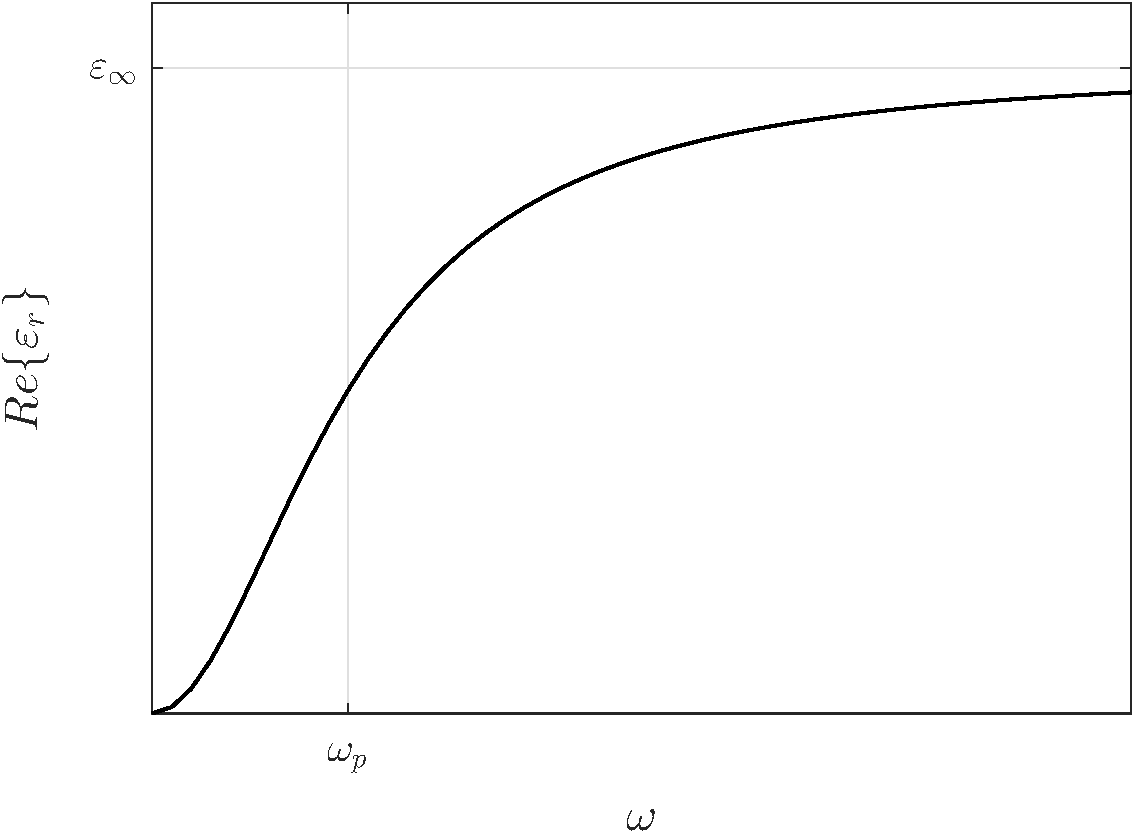
\includegraphics[width=\linewidth]{Figures/Chapters/PhysicalProblem/drudePermittivityReal}
  \captionof{figure}{First caption}
  \label{img1}
\end{minipage}
\hspace{.05\linewidth}
\begin{minipage}{.45\linewidth}
  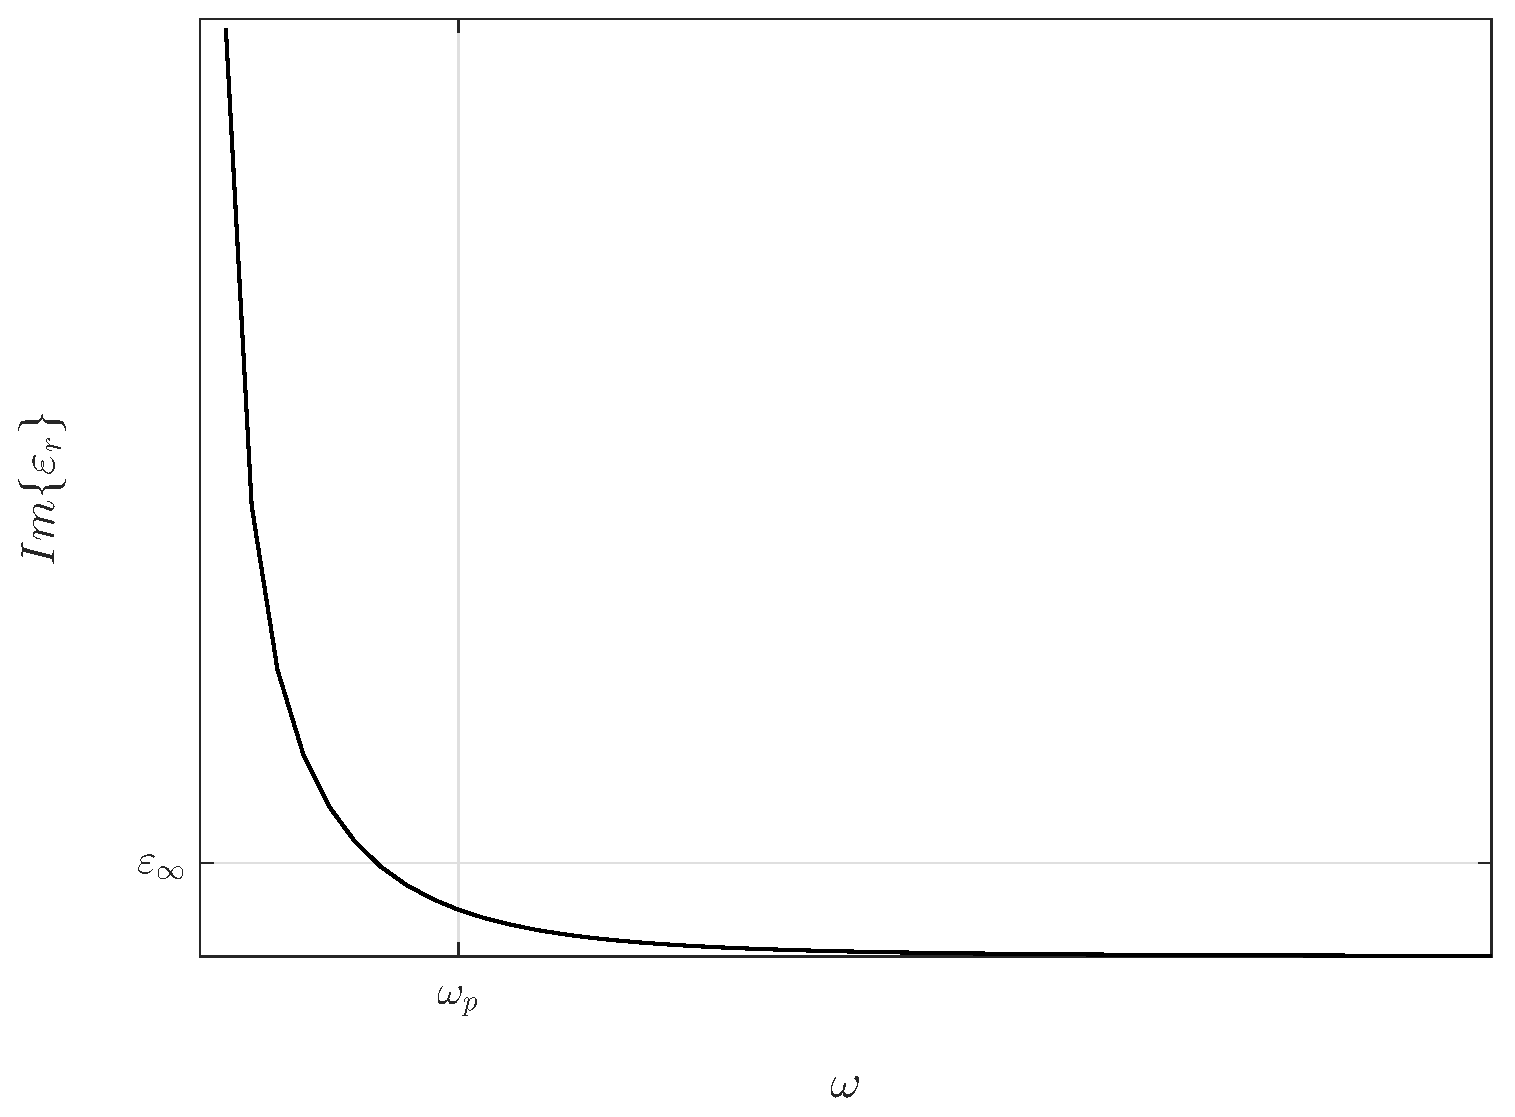
\includegraphics[width=\linewidth]{Figures/Chapters/PhysicalProblem/drudePermittivityImag}
  \captionof{figure}{Second caption}
  \label{img2}
\end{minipage}
\end{figure}
}


\usepackage{xparse}

\ExplSyntaxOn
% Usage:
% \twoimages{
%     {Chapters/figure/path}{figure caption},
%     {Chapters/figure/path}{another caption}
% }
\NewDocumentCommand{\twoimages}{ >{ \SplitList {,} } m }
 {
  \centering
  \ProcessList { #1 } { \__davs_process_argument:n }
 }
\cs_new_protected:Nn \__davs_process_argument:n
 {
  \__davs_image:nnn #1
 }
\cs_new_protected:Nn \__davs_image:nnn
 {
  \begin{subfigure}{0.45\textwidth}
    \centering
    \includegraphics[width=\textwidth]{Figures/#1}
    %\caption{#2}
    %\label{ris:#1}
  \end{subfigure} %
  \hfill
  \penalty0 % we provide a break point
 }
\ExplSyntaxOff
%%% Local Variables:
%%% mode: latex
%%% TeX-master: t
%%% End:
